\documentclass{beamer}

% Setup appearance:

% \usetheme{Darmstadt}
% \usefonttheme[onlylarge]{structurebold}
% \setbeamerfont*{frametitle}{size=\normalsize,series=\bfseries}
\setbeamertemplate{navigation symbols}{}

\begin{document}

\begin{frame}{A divergence operator on icosehedral grids}
  \begin{figure}[htbp]
  \centering
  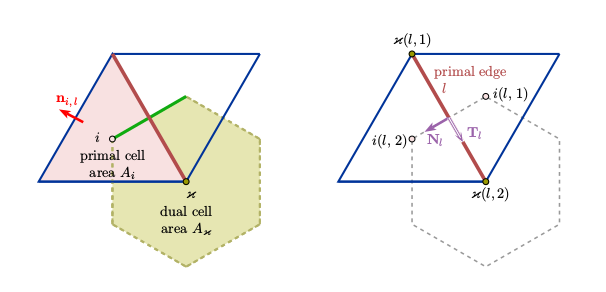
\includegraphics[width=0.8\textwidth]{1.png}
  % \caption{pic}
  % \label{fig:myphoto}
  \end{figure}
  \[\text{div}(v)_i = \frac{1}{A_i}\sum\limits_{l\in \mathcal{E}(i)}v_{n_l}(N_l \cdot n_{i,l})l\]
\end{frame}

\begin{frame}[fragile]{ICON Fortran}
  how to do a div?
\end{frame}

\begin{frame}{GridTools}
  in a similar fashion
\end{frame}

\begin{frame}{GridTools}
How to get edges\%primal\_edge\_length and cells\%area?

\hspace{5em}

netCDF file and a converter.
\end{frame}

\begin{frame}{GridTools}
  and signs?
\end{frame}

\begin{frame}{Next}
  \begin{itemize}
    \item average divergence $\overline{\Big(\text{div}(v)_0\Big)}$: a nested operator
    \item laplacian $(\nabla^2_dv)_l\cdot N_l=\text{grad}_n[\text{div}(v)]_l-\text{grad}_\tau[\text{curl}(v)]_l$
    : nested and fusion
    \item fourth-order hyper-Laplacian $\nabla^4_dv=\nabla^2_d(\nabla^2_dv)$
  \end{itemize}
\end{frame}
\end{document}
